% DPF 09 talk on strangeness in nucleon

\documentclass[10pt]{beamer}
\usepackage{amsmath}
\usepackage{mathtools}
%\documentclass[12pt]{beamerthemeSam.sty}
\usepackage{epsf}
%\usepackage{pstricks}
%\usepackage[orientation=portrait,size=A4]{beamerposter}
\geometry{paperwidth=160mm,paperheight=120mm}
%DT favorite definitions
\def\LL{\left\langle}	% left angle bracket
\def\RR{\right\rangle}	% right angle bracket
\def\LP{\left(}		% left parenthesis
\def\RP{\right)}	% right parenthesis
\def\LB{\left\{}	% left curly bracket
\def\RB{\right\}}	% right curly bracket
\def\PAR#1#2{ {{\partial #1}\over{\partial #2}} }
\def\PARTWO#1#2{ {{\partial^2 #1}\over{\partial #2}^2} }
\def\PARTWOMIX#1#2#3{ {{\partial^2 #1}\over{\partial #2 \partial #3}} }

\def\rightpartial{{\overrightarrow\partial}}
\def\leftpartial{{\overleftarrow\partial}}
\def\diffpartial{\buildrel\leftrightarrow\over\partial}

\def\BI{\begin{itemize}}
\def\EI{\end{itemize}}
\def\BE{\begin{displaymath}}
\def\EE{\end{displaymath}}
\def\BEA{\begin{eqnarray*}}
\def\EEA{\end{eqnarray*}}
\def\BNEA{\begin{eqnarray}}
\def\ENEA{\end{eqnarray}}
\def\EL{\nonumber\\}


\newcommand{\map}[1]{\frame{\frametitle{\textbf{Course map}}
\centerline{\includegraphics[height=0.86\paperheight]{../../map/#1.png}}}}
\newcommand{\wmap}[1]{\frame{\frametitle{\textbf{Course map}}
\centerline{\includegraphics[width=0.96\paperwidth]{../../map/#1.png}}}}

\newcommand{\etal}{{\it et al.}}
\newcommand{\gbeta}{6/g^2}
\newcommand{\la}[1]{\label{#1}}
\newcommand{\ie}{{\em i.e.\ }}
\newcommand{\eg}{{\em e.\,g.\ }}
\newcommand{\cf}{cf.\ }
\newcommand{\etc}{etc.\ }
\newcommand{\atantwo}{{\rm atan2}}
\newcommand{\Tr}{{\rm Tr}}
\newcommand{\dt}{\Delta t}
\newcommand{\op}{{\cal O}}
\newcommand{\msbar}{{\overline{\rm MS}}}
\def\chpt{\raise0.4ex\hbox{$\chi$}PT}
\def\schpt{S\raise0.4ex\hbox{$\chi$}PT}
\def\MeV{{\rm Me\!V}}
\def\GeV{{\rm Ge\!V}}

%AB: my color definitions
%\definecolor{mygarnet}{rgb}{0.445,0.184,0.215}
%\definecolor{mygold}{rgb}{0.848,0.848,0.098}
%\definecolor{myg2g}{rgb}{0.647,0.316,0.157}
\definecolor{abtitlecolor}{rgb}{0.0,0.255,0.494}
\definecolor{absecondarycolor}{rgb}{0.0,0.416,0.804}
\definecolor{abprimarycolor}{rgb}{1.0,0.686,0.0}
\definecolor{Red}           {cmyk}{0,1,1,0}
\definecolor{Grey}           {cmyk}{.7,.7,.7,0}
\definecolor{Blue}          {cmyk}{1,1,0,0}
\definecolor{Green}         {cmyk}{1,0,1,0}
\definecolor{Brown}         {cmyk}{0,0.81,1,0.60}
\definecolor{Black}         {cmyk}{0,0,0,1}

\usetheme{Madrid}


%AB: redefinition of beamer colors
%\setbeamercolor{palette tertiary}{fg=white,bg=mygarnet}
%\setbeamercolor{palette secondary}{fg=white,bg=myg2g}
%\setbeamercolor{palette primary}{fg=black,bg=mygold}
\setbeamercolor{title}{fg=abtitlecolor}
\setbeamercolor{frametitle}{fg=abtitlecolor}
\setbeamercolor{palette tertiary}{fg=white,bg=abtitlecolor}
\setbeamercolor{palette secondary}{fg=white,bg=absecondarycolor}
\setbeamercolor{palette primary}{fg=black,bg=abprimarycolor}
\setbeamercolor{structure}{fg=abtitlecolor}

\setbeamerfont{section in toc}{series=\bfseries}

%AB: remove navigation icons
\beamertemplatenavigationsymbolsempty
\title[Friction (etc.)]{
  \textbf {Friction (and sundry)}\\
%\centerline{}
%\centering
%\vspace{-0.0in}
%\includegraphics[width=0.3\textwidth]{propvalues_0093.pdf}
%\vspace{-0.3in}\\
%\label{intrograph}
}

\author[W. Freeman] {Physics 211\\Syracuse University, Physics 211 Spring 2015\\Walter Freeman}

\date{\today}

\begin{document}

\frame{\titlepage}

\frame{\frametitle{\textbf{Announcements}}
\BI
\Large
\item{Homework 4 extended until Friday}
\item{{\it Mastering Physics} assignment due Thursday}
\item{Read Chapter 8}
  \pause
\item{Exam date change: {\it let me know} if there's a problem with moving it}
  \BI
\item{Feb 26 $\rightarrow$ March 3}
\EI
\EI

}

\frame{\frametitle{\textbf{Ask a Physicist: How does an airplane work?}}

}


\frame{\frametitle{\textbf{Homework review: Two objects moving}}
  \BI
\item{Demo: Atwood's machine}
\item{Same as always: Force diagram $\rightarrow$ Newton's law for each object $\rightarrow$ solve}
\item{Two different objects $\rightarrow$ two different accelerations!}
\EI
\large
\centerline{$T_1-m_1g = m_1 a_1$}
\centerline{$T_2-m_2g = m_2 a_2$}
\pause

\bigskip
\bigskip

\centerline{$T_1 = T_2$}
\pause

\bigskip
\bigskip

\centerline{$a_1 = -a_2$ (``standard coordinate system'')}
\centerline{$a_1 = a_2$ (``reverse coordinate system'')}
}

\frame{\frametitle{\textbf{Rotational motion}}
\Large
Often things in nature are constrained to go in circles:

\begin{itemize}
  \item{Planets orbiting stars; moons orbiting planets (close enough to circles)}
  \item{Wheels; things on strings; many others}
\end{itemize}

\bigskip
\bigskip

We'll study ``{\color{Blue}uniform }{\color{Red} circular motion}'' here: 

\begin{itemize}
  \item{Something moves at a {\color{Red}constant distance} from a fixed point}
  \item{... at a {\color{Blue}constant speed}.}
\end{itemize}

}


\frame{\frametitle{\textbf{Rotational motion: description}}
  \begin{itemize}
    \item{Object moves in a circle of radius $r$, with its angle changing at a constant rate}
    \item{``Position = rate $\times$ time'' $\rightarrow$ ``Angle = rate $\times$ time''}
  \end{itemize}

\pause

  \Large
\centerline{$\theta = \omega t$}
\large

\bigskip

\centerline{$\omega$ (omega) called the ``angular velocity''; measured in radians per second}

\begin{itemize}
  \item{Angular velocity tells you how fast something spins: RPM's are another unit}
  \item{A larger radius does {\it not} mean something has a higher angular velocity}
\end{itemize}
}

\frame{\frametitle{\textbf{Rotational motion: description}}
  \Large Some new terms:
  \large
  \begin{itemize}
    \item{``Radial'': directed in and out of the circle}
    \item{``Tangential'': directed around the circle}
    \item{The radial velocity is 0 ($r$ doesn't change)}
    \item{The tangential velocity depends on $r$ and $\omega$, as you'd expect}
  \end{itemize}
}

\frame{\frametitle{\textbf{Radians}}
  \large

  The radian: new unit of angle. $2\pi$ radians = 360 degrees.

  \bigskip

  1 complete circle is $2\pi$ radians; 1 complete circumference is $2\pi$ radiuses ($C = 2\pi r$).

  1 radian thus has an arc length of 1 radius.

  $\theta$ radians therefore have an arc length of $r \theta$.
  
\bigskip

  \hspace{0.1\textwidth}
  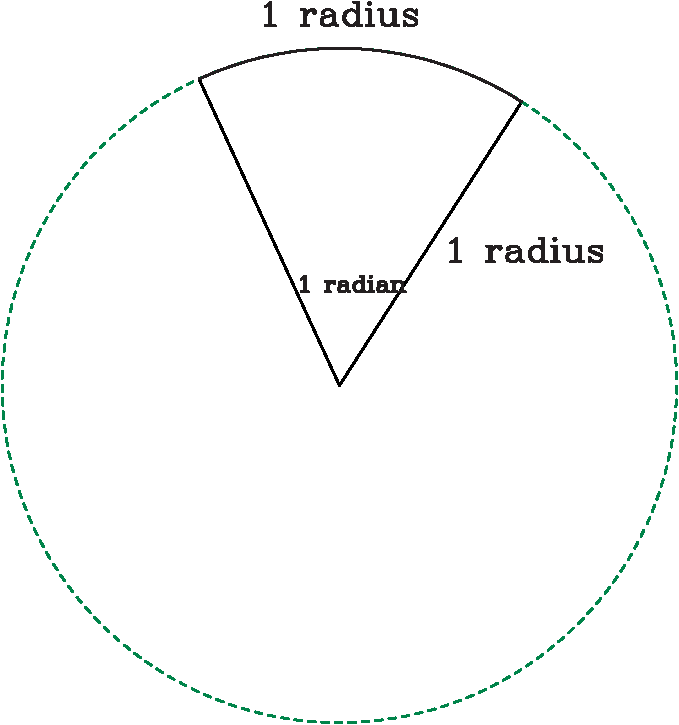
\includegraphics[width=0.30\textwidth]{circle1-crop.pdf}\hspace{0.15\textwidth}
  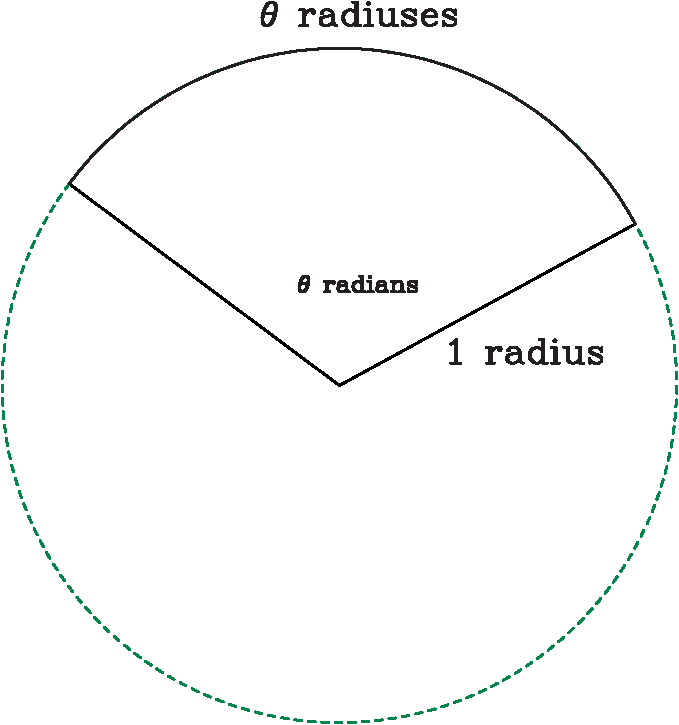
\includegraphics[width=0.30\textwidth]{circle2-crop.pdf}

\bigskip

  \centerline{\color{Red}$\rightarrow$ Tangential movement (in meters) = angular movement (in radians) times the radius}

}


\frame{\frametitle{\textbf{Rotational motion: description}}
  \Large Some new terms:
  \large
  \begin{itemize}
    \item{``Radial'': directed in and out of the circle}
    \item{``Tangential'': directed around the circle}
    \item{The radial velocity is 0 ($r$ doesn't change)}
    \item{The tangential velocity depends on $r$ and $\omega$, as you'd expect}
      \pause
    \item{$v_T = \omega r$: ``meters per second = radians per second times meters per radian''}
  \end{itemize}
}


\frame{\frametitle{\textbf{Kinematic challenge: what's the acceleration}}
\Large

Clearly an object moving in a circle is accelerating. What's the acceleration?

  \hspace{0.1\textwidth}
  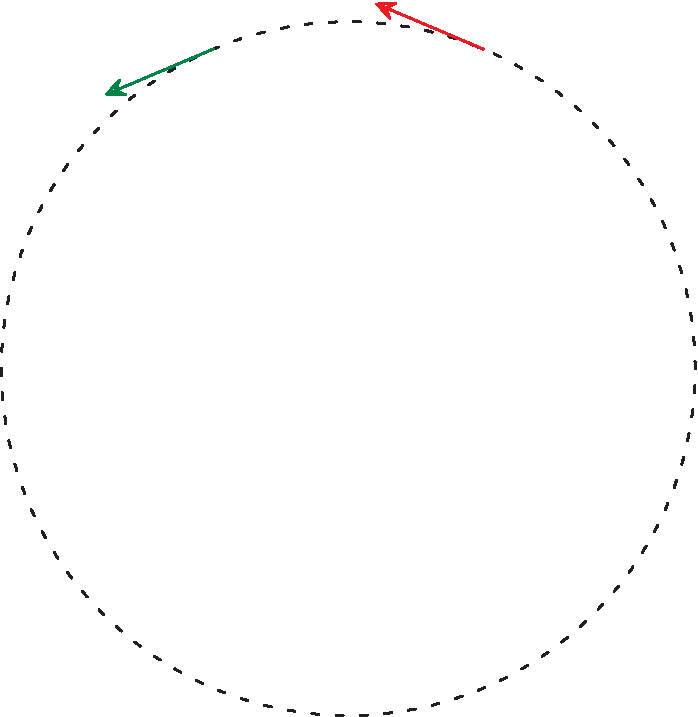
\includegraphics[width=0.30\textwidth]{acc1-crop.pdf}\hspace{0.15\textwidth}
  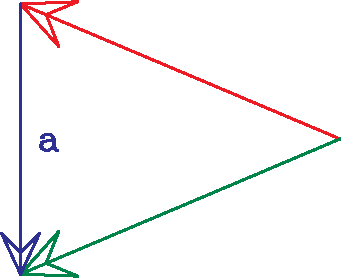
\includegraphics[width=0.30\textwidth]{acc2-crop.pdf}


\bigskip
  
  \large
\pause

Near the top of the circle, the $y$-component of the velocity decreases; we expect then that $\vec a$ points downward.

\bigskip

Can we make this rigorous?

}


\frame{\frametitle{\textbf{Some math}}
\large

$x(t) = r \cos (\omega t)$
$y(t) = r \sin (\omega t)$

\pause

\bigskip
\bigskip

Differentiate to get $v_x$ and $v_y$:

\bigskip

$v_x(t) = -\omega r \sin (\omega t)$

$v_y(t) = \,\,\,\,\omega r \cos (\omega t)$

\pause

\bigskip
\bigskip

Differentiate again to get $a_x$ and $a_y$:

\bigskip

$a_x(t) = -\omega^2 r \cos (\omega t) = -\omega^2 x(t)$

$a_y(t) = -\omega^2 r \sin (\omega t) = -\omega^2 y(t)$

\pause

\bigskip
\bigskip

$\rightarrow \vec a = -\omega^2 \vec r$

\bigskip
\pause

{\color{Red}An object in uniform circular motion accelerates toward the center of the circle with }

\bigskip

\centerline{  \color{Green}$\rightarrow a=\omega^2 r=v^2/r \leftarrow $}
}

\frame{\frametitle{\textbf{Uniform circular motion, consequences}}
  \large
  If you know an object is undergoing uniform circular motion, you know something about the acceleration:

\bigskip

\centerline{\color{Red} $a=\omega^2 r$ or $a=v^2/r$ toward the center of the circle.}

\bigskip

\pause

Circular motion problems aren't scary; they are just like equilibrium problems.

\begin{itemize}
  \item{Equilibrium problem: $\sum F_x = ma_x = 0$ and $\sum F_y = ma_y = 0$}
  \item{Circular motion problem: $\sum F_T = ma_T = 0$ and $\sum F_r = ma_r = v^2/r$}
  \end{itemize}

  \bigskip

  $\rightarrow$ If we tell you that a thing is in uniform circular motion, we're just telling you something about its acceleration.

}

\frame{\frametitle{\textbf{Centripetal force}}
  \large
  ``Centripetal'' means ``toward the center'' in Latin.

\bigskip
\BI
\item{If something is going to accelerate toward the center, a force must do that.}

\item{Centripetal force is {\color{Red} not} a ``new'' force. No arrows labeled ``centripetal force''!}

\item{``Centripetal'' is a word that describes a force you already know about.}
\item{Centripetal force: describes a force that holds something in a circle}


\item{It can be lots of things:}
  \BI
  \normalsize
\item{Tension (stuffed animal on a string demo)}
\item{Normal force (platform, bucket demos)}
\item{Friction (Ferris wheel)}
\item{Gravity (the moon!)}
  \EI
  \EI
}






\frame{\frametitle{\textbf{Sample problems}}

  (from demos)
}



\end{document}
